%\chapter{Proof of Concept Design and Implementation}
%\chapter{Pixel-based Synthesis of 360\degree Viewpoints}
\chapter{Pixel-based Synthesis of 360\degree Viewpoints with 2DoF}\label{chap:implementation}

\ldots The different appraches to image-based rendering presented in the previous chapter use different assumptions and simplifications of the plenoptic function in order to facilitate its reconstruction. Most of these approaches are based on planar images, which already significantly reduces the complexity of the data to be processed. The approach presented here, on the other hand, works on 360\degree images, which increases data processing and storage. As a result, other assumptions and simplifications are made, the most prominent being the exemption of scene geometry, and the limitation to two degrees of freedom (2DoF). Limiting movement to 2DoF means that the location of possible synthesized points is restricted to a plane. 

This chapter presents the assumptions and simplifications made for the pixel-based synthesis of 360\degree viewpoints, the basic approach and an improvement to the basic approach based on flow-based blending from Richardt et al.'s Megastereo \cite{megastereo}, and the implementation details of the method.

\section{Approach} \label{sec:approach}
%\begin{itemize}
%  \item most other approaches rely on either geometry or correspondences
%  \item usually some form of triangulation
%  \item use of sphere for ray tracing, then use texture lookup to find the pixel values
%  \item combination of reprojection ie warping with angle constraint and flow-based blending
%  \item first part relies on radius/scale, but no geometry, second part relies on image correspondences
%  \item ``view-dependent texture maps'' \ar environment map / viewpoint is chosen based on some kind of proximity to the synthesized view
%  \item pixel-based, in that each pixel is calculated separately, there are not image-area based constraints
%\end{itemize}

\subsection{Assumptions}
In order to simplify the process of synthesis, some assumptions are made based on the scene and the viewpoints in the scene:

\begin{itemize}
  \item the scene is static
  \item all images are captured on a plane parallel to the floor (viewpoint plane)
  \item all synthesized viewpoints are located inside the scene boundaries and are also located on the viewpoint plane
  \item the positions and orientations of the captures are known
  \item the scale (max radius) of the scene is known
\end{itemize}

Furthermore, for the moment, it is assumed that the optical flow algorithm used in the flow-based blending calculates a decent result between any pair of viewoints.

\subsection{Basic 2DoF Synthesis} \label{subsec:basic-synthesis}
With these assumptions and using a basic model geometry with approximately the same scale as the captured scene, it is already possible to synthesize new viewpoints with varying accuracy, depending on the scene. The process presented here for basic 2DoF synthesis is a combination of texture lookup through raytracing, and mosaicking by using a constraint based on the ray deviation angle.

\subsubsection{Raytracing-based Texture Lookup}
The first step is to map the texture (i.e. pixel values) of an existing viewpoint to a new viewpoint according to its position in the scene. Theoretically, any 360\degree viewpoint can be mapped to any other, since each 360\degree image captures each point in the scene. This is only theoretically the case, since image resolution and occlusions in the scene will conceal some areas for some viewpoints whereas they are visible for others. However, at this point, this will be ignored and it will be assumed that each viewpoint image contains all the points of the scene albeit at different image coordinates and different sampling rates\footnote{By design, areas closer to the camera are captured with a higher sampling rate per point than areas farther away.}. 

Additionally, 3D geometry of the scene is needed for raytracing. However, since the approach in this thesis does not capture or infer any real geometry, a model geometry is used that has approximately the same scale as the scene that was captured. The model geometry is a sphere, as this is a simple, very general geometry to represent a variety of different scenes. The radius of the sphere is chosen so that the sphere contains all possible points in the scene, for which the scale of the scene needs to be known. Under these assumptions, it is possible to map the image at one viewpoint to a new position by combining raytracing and texture lookup.

% This is visualized in Figure~\ref{fig:reflected_rays} a: Each point P of the scene reflects light rays in all directions. These light rays are captured at different viewpoints and are discretized into pixels in the image taken at that viewpoint. As a result, the pixels representing point P are present in the images captured at each viewpoint. This means that when synthesizing a new viewpoint S, the pixels representing point P can theoretically be retrieved from any of the images at the captured viewpoints (Figure~\ref{fig:reflected_rays} b).
%\begin{figure}[]
%\centering
%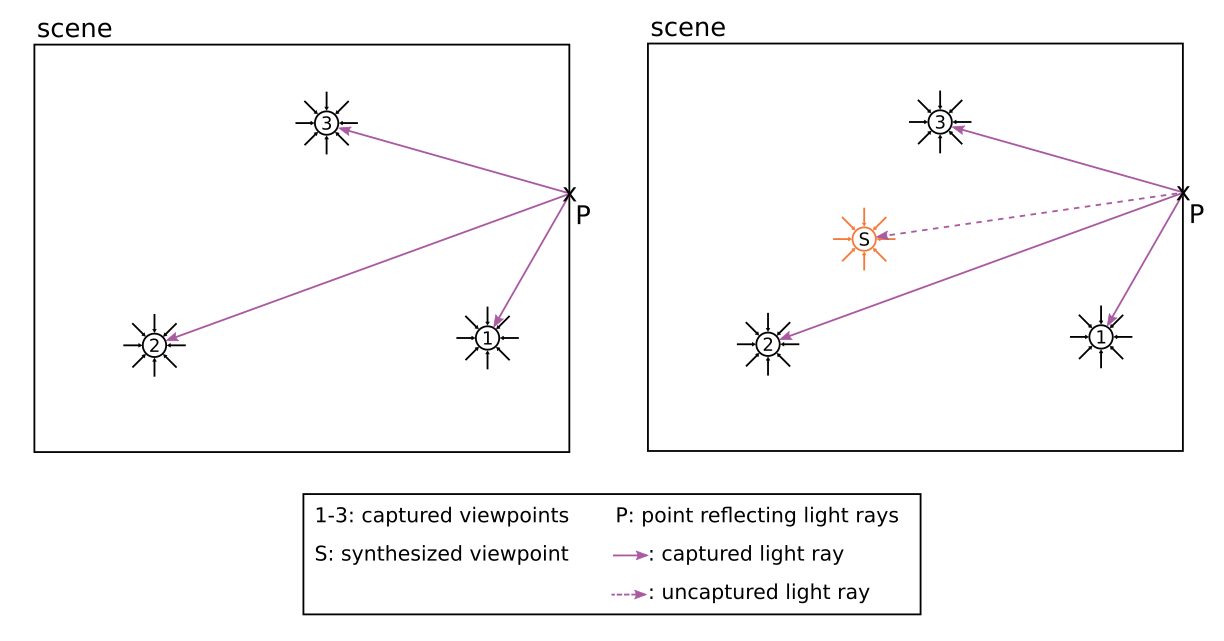
\includegraphics[width=1\textwidth]{03/incoming_lightrays.png}
%\caption[Light rays reflected from a point in the scene]{The reflected light rays from each point in the scene are captured by each 360\degree viewpoint}
%\label{fig:reflected_rays}
%\end{figure}

In order to do this, several steps of raytracing are necessary, which are visualized in Figure~\ref{fig:raytracing}. Figure~\ref{fig:raytracing}a shows how a camera at a specific viewpoint captures the light rays reflected from the objects in the scene. The captured pixel values are visualized on a circle around the center of projection of the camera (for simplicity's sake, only one row of pixels is shown). Once the viewoints have been captured (there is only one viewpoint in this example), a new viewpoint is ready to be synthesized. The model geometry is visualized as a circle\footnote{In this example, the model sphere does not surround the complete scene (the corners of the scene are outside of the circle). This is only for visualization purposes, normally the sphere would contain the complete scene, including the corners.} in Figure~\ref{fig:raytracing}b, with the new viewpoint to be synthesized represented by a dotted circle around a center of projection. For each pixel of the synthesized image, a ray is projected into the scene (Figure~\ref{fig:raytracing}c) and its intersection with the scene is calculated. Then, the ray from the center of projection of the captured viewpoint to the scene intersection is calculated and the pixel value at that position in world coordinates is retrieved (Figure~\ref{fig:raytracing}e) and copied back to the new viewpoint (Figure~\ref{fig:raytracing}f). This way, the pixel values (i.e. texture) of a captured viewpoint are mapped to the new viewpoint (Figure~\ref{fig:raytracing}g). Figure~\ref{fig:raytracing}h compares the mapped values to the actual scene. It is immediately visible that most points have the value they would have, had the viewpoint been captured instead of synthesized (ground truth value), whereas some are incorrect. This is due to the disparity between the model and the real scene.

\begin{figure}
\centering
    \hfill
    \begin{subfigure}[t]{0.3\textwidth}            
            \centering
            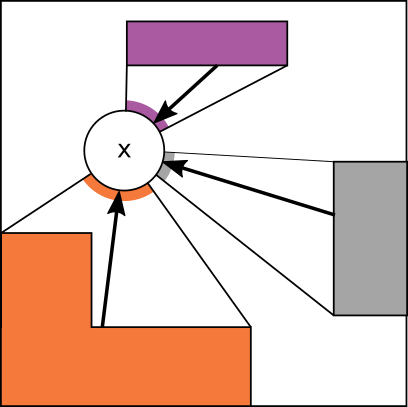
\includegraphics[width=0.9\textwidth]{03/raytracing01.png}
            \caption{The real scene viewed from above: The camera captures light rays reflecting from objects}
    \end{subfigure}%
    \hfill
     %add desired spacing between images, e. g. ~, \quad, \qquad etc.
      %(or a blank line to force the subfigure onto a new line)
    \begin{subfigure}[t]{0.3\textwidth}
            \centering
            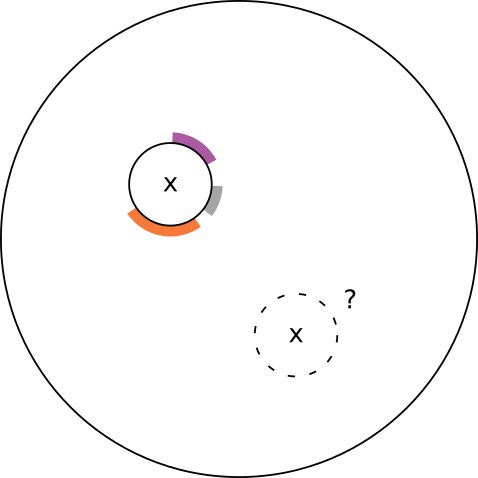
\includegraphics[width=0.9\textwidth]{03/raytracing02.png}
            \caption{A new viewpoint to be synthesized using the model geometry (sphere)}
    \end{subfigure}
    \hfill
    \hfill

    \hfill
    \begin{subfigure}[t]{0.3\textwidth}            
            \centering
            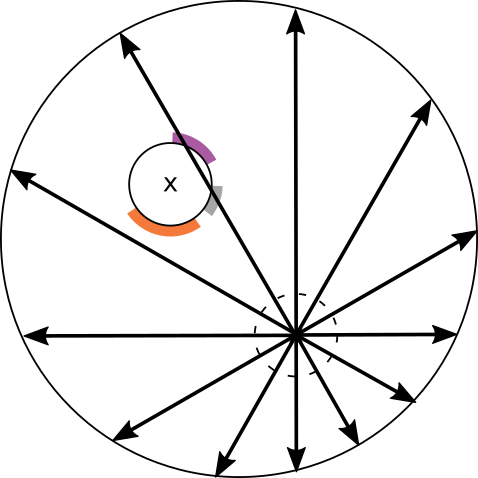
\includegraphics[width=0.9\textwidth]{03/raytracing03.png}
            \caption{A ray for each pixel in the synthesized viewpoint is traced to its intersection with the model}
    \end{subfigure}%
    \hfill
    \begin{subfigure}[t]{0.3\textwidth}
            \centering
            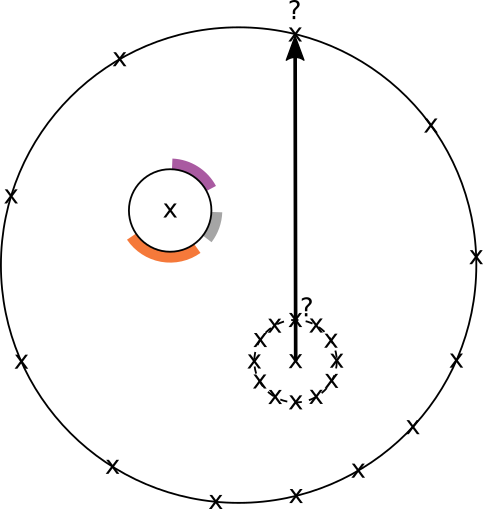
\includegraphics[width=0.9\textwidth]{03/raytracing04.png}
            \caption{For each ray, a texture lookup is performed}
    \end{subfigure}
    \hfill
    \begin{subfigure}[t]{0.3\textwidth}
            \centering
            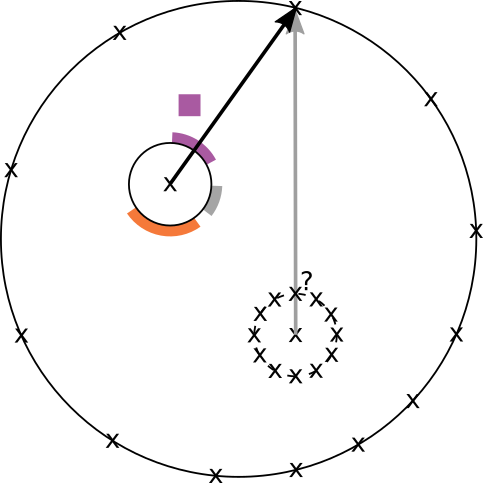
\includegraphics[width=0.9\textwidth]{03/raytracing05.png}
            \caption{From the ray-model intersection, a second ray is traced to the center of projection of the captured viewpoint and the pixel value is looked up}
    \end{subfigure}
    \hfill

    \hfill
    \begin{subfigure}[t]{0.3\textwidth}            
            \centering
            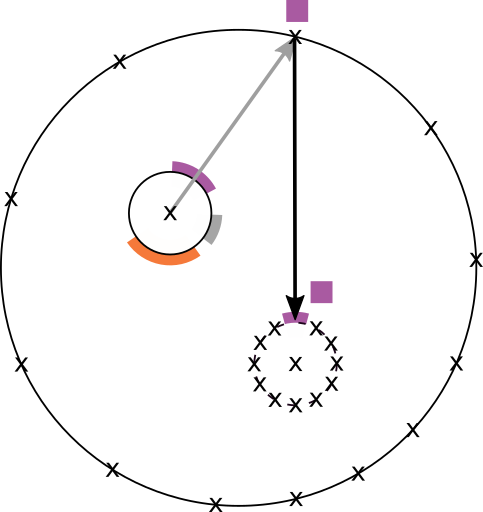
\includegraphics[width=0.9\textwidth]{03/raytracing06.png}
            \caption{The pixel value is copied back to the new viewpoint}
    \end{subfigure}%
    \hfill
    \begin{subfigure}[t]{0.3\textwidth}
            \centering
            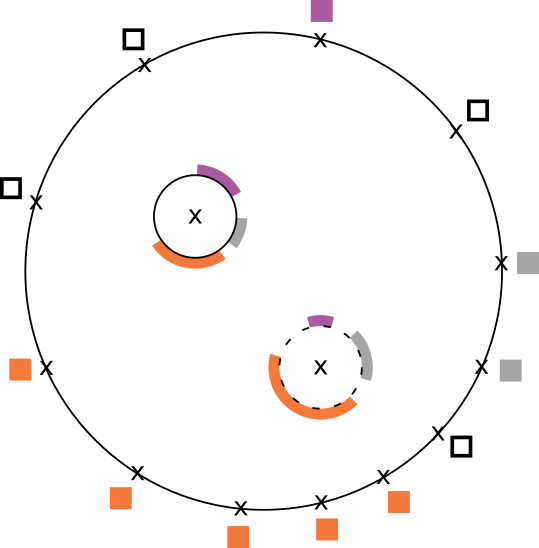
\includegraphics[width=0.9\textwidth]{03/raytracing07.png}
            \caption{This process is repeated for all pixels}
    \end{subfigure}
    \hfill
    \begin{subfigure}[t]{0.3\textwidth}
            \centering
            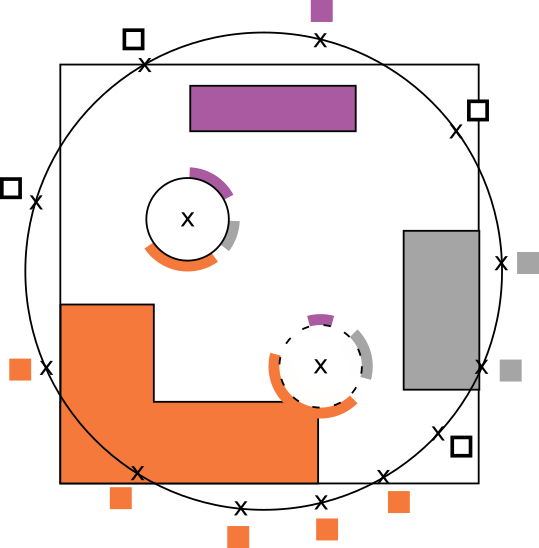
\includegraphics[width=0.9\textwidth]{03/raytracing08.png}
            \caption{The resulting texture mapping from the captured viewpoint to the model geometry in comparison with the original scene}
    \end{subfigure}
    \hfill
    \caption[Texture lookup through raytracing]{Process of texture lookup through raytracing}\label{fig:raytracing}
\end{figure}

%The basic idea of the 2/3DoF algorithm is to find the image areas from the set of existing viewpoints that are the ``most fitting'' for the synthesized viewpoint and transform these areas to approximate where they would be in the synthesized image. This means that a metric is necessary that measures how ``fitting'' a specific pixel of a viewpoint image is. Also, a reprojection needs to be found that transforms the ``fitting'' image areas to the appropriate image coordinates for the synthesized viewpoint.
%\missingfigure{point correspondences and reprojection intro}


\subsubsection{Deviation-angle-based Mosaicking}
The example in Figure~\ref{fig:raytracing} contains only one captured viewpoint, so the choice of which viewpoint to use for texture lookup is trivial. In cases where several viewpoints are available, a choice must be made as to which viewpoint should be used. In the case where the real scene has the same geometry as the model sphere, this is practically irrelevant, since the raytracing is always accurate. However, this is unrealistic, since the number of spherical rooms containing no objects is negligible. As a result, as soon as the real scene differs from the model sphere, some viewpoints yield better results than others. Figure~\ref{fig:dev_angle}a shows how a discrepancy between the real scene and the model sphere can lead to inaccurate results.

When comparing rays from different viewpoints, two metrics can be examined: the euclidean distance of the captured viewpoint from the synthesized viewpoint, and the deviation angle between the rays. Figure~\ref{fig:dev_angle}b visualizes the two metrics and in the example, the $vp2$ with the smaller deviation angle is a better match. In fact, assuming that there is no obscuring element in the air such as fog, and disregarding diffusion and scattering over distance, the same light ray is captured by any viewpoint located on the ray in question. This means the closer the deviation angle is to zero, the more accurate the result will be, no matter the distance of the viewpoints. However, sampling rates and resolution also have an effect on the sampled point, so the euclidean distance cannot be completely ignored. \todo{put a third image in fig 3.2 to illustrate the deviation angle 0}

Instead of combining these metrics in a function that might have to be weighted differently depending on the scene size, the distribution viewpoints, and more, the choice of which viewpoints to use is divided into two different steps: The choice of input viewpoints from all captured viewpoints for the synthesis of a specific point, and the choice of which of the input viewpoints to use for each ray of the synthesized point. 

The pre-selection of input viewpoints from all captured viewpoints is based on the assumption that the closer the captured viewpoints are to the synthesized viewpoint, the more accurate the sampling of the surroundings will be (i.e. the relative size of the objects). As a result, all viewpoints further than a certain distance are discarded from the input.

After selecting the most appropriate captured viewpoints, the synthesized image is created by comparing the deviation angles of these viewpoints for each ray (i.e. pixel). The two closest viewpoints are then blended together on a per-pixel basis, so that there are no abrupt edges between mosaic areas. The blending function and is presented in more detail in Section~\ref{sec:impl_details}.
%depending on the number and relative location of the captured viewpoints, using a per-pixel, deviation-angle-based constraint leads to a synthesized image made up of patches from different viewpoints (i.e. mosaic). 

\begin{figure}
\centering
    \hfill
    \begin{subfigure}[t]{0.3\textwidth}            
            \centering
            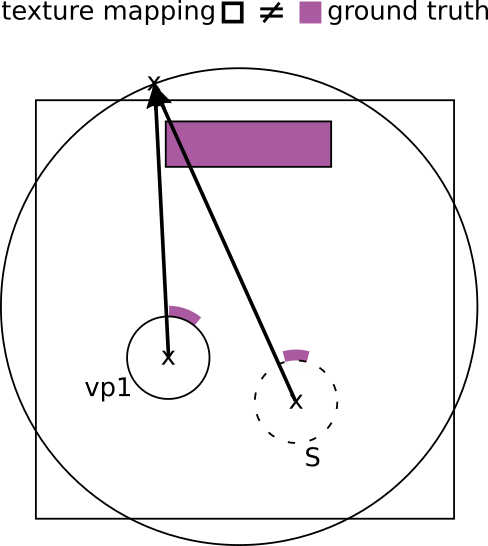
\includegraphics[width=0.9\textwidth]{03/dev_angles01.png}
            \caption{Differences in the real scene from the model can lead to inaccurate texture mappings}
    \end{subfigure}%
    \hfill
     %add desired spacing between images, e. g. ~, \quad, \qquad etc.
      %(or a blank line to force the subfigure onto a new line)
    \begin{subfigure}[t]{0.3\textwidth}
            \centering
            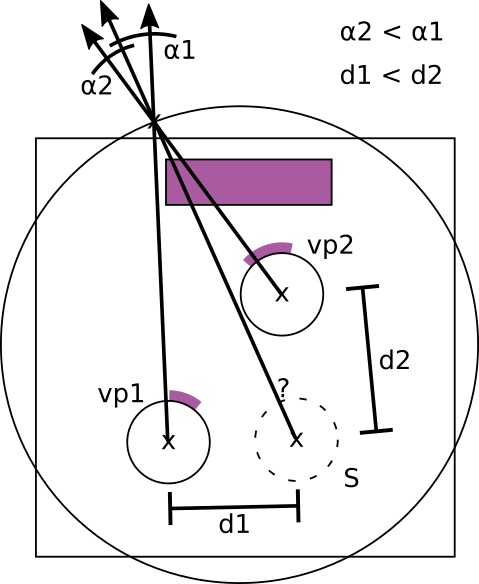
\includegraphics[width=0.9\textwidth]{03/dev_angles02.png}
            \caption{The deviation angle $\alpha$ of the rays can be compared, as well as the euclidean distance d}
    \end{subfigure}
    \hfill
    \hfill
    \caption[Choosing the appropriate viewpoint for texture lookup]{Choosing the appropriate viewpoint to improve the result} \label{fig:dev_angle}
\end{figure}
%In order to find the ``most fitting'' image area from all of the viewpoint images, there first needs to be a metric that measures how ``fitting'' an image area is. 

%One example is the euclidean distance of the viewpoint locations in space. This would mean that for each pixel, the corresponding pixel of the \emph{nearest viewpoint} would be used. This is the simplest approach, and would simply return the nearest neighbor. 

\subsection{2DoF Synthesis using Flow-based Blending}
Using basic 2DoF Synthesis works fairly well as long as the real scene geometry corresponds roughly to the model sphere. The basic shape of many rooms can be approximated by a sphere, however the objects within these rooms can diverge greatly from the model geometry. In these cases, ghosting and doubling artefacts become visible, such as areas appearing twice, not at all, or two areas overlapping inconsistently. This problem is exacerbated when the synthesized viewpoint is very close to an object, as is visualized in Figure~\ref{fig:flow-based-mot}: In this example the synthesized viewpoint is very close to a detailed object whose geometry diverges significantly from the model sphere. The values of the points captured by the two viewpoints $vp1$ and $vp2$ differ (orange and purple), and neither of them is the desired ground truth value (gray) (Figure~\ref{fig:flow-based-mot}a). In order to improve the result, an adapted variation of the flow-based blending method from Richardt et al.'s al.'s Megastereo \cite{megastereo} is introduced. This method allows interpolation between two 360\degree viewpoints using optical flow. Figure~\ref{fig:flow-based-mot}b shows how the interpolation can be used to achieve a more accurate result: A new viewpoint $vp$1-2 is interpolated between $vp1$ and $vp2$ such that the interpolated viewpoint is located on the ray in question\footnote{Positioning the interpolated viewpoint directly on the ray is only possible for rays that are on the 2D plane containing all the viewpoints. All other cases must be approximated.} This new viewpoint is then used for the texture lookup to create the synthesized image with the goal of improving the accuracy of the mapped point.

\begin{figure}
\centering
    \hfill
    \begin{subfigure}[t]{0.4\textwidth}            
            \centering
            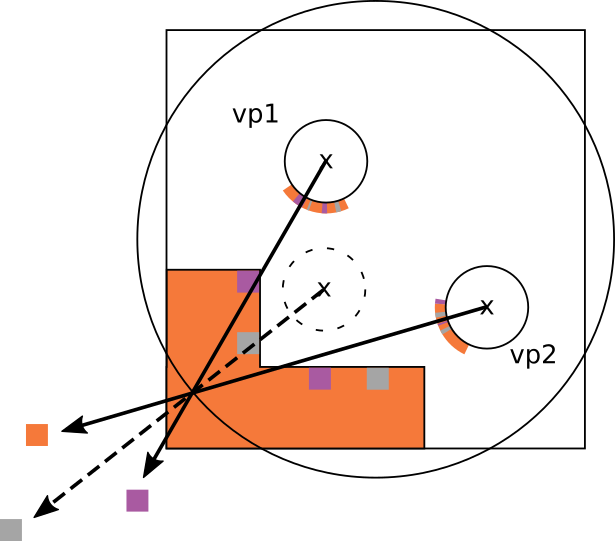
\includegraphics[width=0.9\textwidth]{03/flow-based01.png}
            \caption{Detailed areas where real geometry is very different from the model are problematic for basic 2DoF Synthesis}
    \end{subfigure}%
    \hfill
     %add desired spacing between images, e. g. ~, \quad, \qquad etc.
      %(or a blank line to force the subfigure onto a new line)
    \begin{subfigure}[t]{0.4\textwidth}
            \centering
            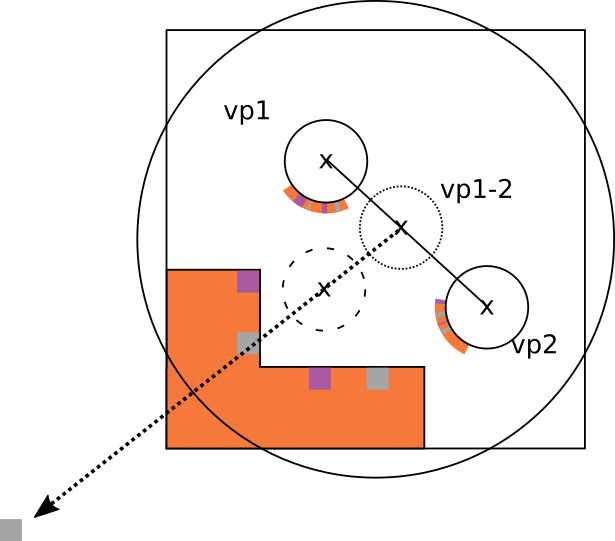
\includegraphics[width=0.9\textwidth]{03/flow-based02.png}
            \caption{Interpolating between input viewpoints using optical flow may improve results}
    \end{subfigure}
    \hfill
    \hfill
  \caption[Flow-based blending to improve accuracy in close, detailed areas]{Introducing flow-based blending to improve accuracy} \label{fig:flow-based-mot}
\end{figure}

%A solution to a similar problem has already been published by Richardt et al. in ``Megastereo'' \cite{megastereo} which introduces an approach using optical flow in order to reduce ghosting artefacts in planar images. The following section shows how the problem of 1D interpolation for 360\degree images can be reduced to the problem solved in Megastereo.

\subsubsection{Adapting Flow-based Blending in Megastereo for 1DoF Interpolation of 360\degree Images}
Megastereo \cite{megastereo} aims to generate high-resolution stereo panoramas by combining images captured on a circle. Their approach is to combine corresponding strips of the captured images and to create a view for each eye (see Section \ref{subsec:megastereo}). In order to mitigate artefacts such as ghosting, they use ``flow-based blending'' to combine two images A and B. This consists of using the optical flow vectors $F_{A\rightarrow B}$ and their inverse $F_{B\rightarrow A}$. To get the interpolated image at position $\delta$ between image A and B, first, image A is shifted by $\delta \cdot F_{A\to B}$ and image B is shifted by $(1 - \delta) \cdot F_{A\to B}$, yielding $I_A$ and $I_B$, respectively. Then, $I_A$ is multiplied by $(1-\delta)$ and $I_B$ by $\delta$ and these pixel values are added together to give the resulting interpolation. This is described by the following function, in which each pixel at position x of the synthesized image S is defined by: 

\begin{align}
S(x) &= (1-\delta ) \cdot A( x + \delta \cdot F_{A\to B}(x)) \nonumber\\
     &\qquad {} + \delta \cdot B( x + (1-\delta) \cdot F_{B\to A}(x)) \label{eq:flow_blending}
   \end{align}

%\subsubsection{Reducing 360\degree Interpolation to Planar Interpolation}
The flow-based blending in Megastereo operates on planar images. In order to use it for 360\degree synthesis, it is necessary to adapt the method for 360\degree images.

A 360\degree image can be projected in several ways, as described in Section \ref{subsec:projections}. The output of these projections is a planar image, meaning that it would be possible to apply flow-based blending directly. However, optical flow algorithms are generally designed to handle planar images without seams or distortions and would most likely produce unexpected results if used naively on planar projections of 360\degree images. As a result, the 360\degree images must first be projected and adapted in such a way that optical flow can be calculated accurately on them.

%Most projections distort the image in some areas, which would result in distorted optical flow values, e.g. the areas towards the poles in the equirectangular projection. Furthermore, in order to make planar viewing possible, the 360\degree image must be ``unfolded'' along some seam. When calculating optical flow, points that move across the seam will not be tracked, even though they do not move out of the image space, as would happen in a regular image.

Of the projections presented in Section~\ref{subsec:projections}, only the cube map representation is applicable. Spherical representations are impractical, as aligning seams is not feasible and the distortion towards the edges is extreme. The equirectangular representation has only four seams to handle, but also distorts the image greatly around the poles. The cube map representation contains a number of seams but does not distort the image more than a planar image would be. 
The challenge presented by the many seams of the cube map is to be able to track points that move across the seams created by the six faces. Figure~\ref{fig:flow_seams} shows an example of different points moving across seams, illustrating why calculating optical flow on each face separately would not be enough. Figure~\ref{fig:flow_seams} also shows the linear discontinuities at the seams (e.g. at the upper edge of the carpet): since each cube face was captured by a different virtual camera, angles are not consistent across seams. As a result it is not possible to use the cube map as it is, since the optical flow assumes linear movement\footnote{Optical flow uses vectors to describe movement, which are inherently linear}.
\todo{use images from 12x12 so that fov can be smaller}

\begin{figure}
\centering
    \hfill
    \begin{subfigure}[t]{0.5\textwidth}            
            \centering
            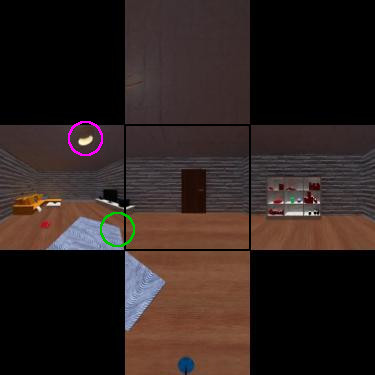
\includegraphics[width=0.9\textwidth]{03/flow_seams01.jpg}
            \caption{Viewpoint A in cube map representation (90\degree FoV per face)}
    \end{subfigure}%
    \hfill
     %add desired spacing between images, e. g. ~, \quad, \qquad etc.
      %(or a blank line to force the subfigure onto a new line)
    \begin{subfigure}[t]{0.5\textwidth}
            \centering
            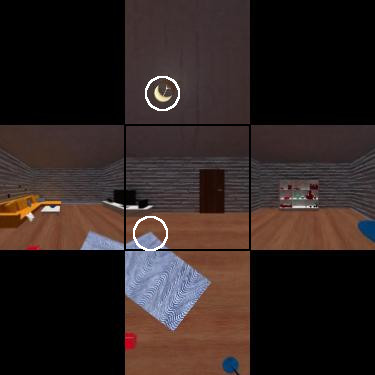
\includegraphics[width=0.9\textwidth]{03/flow_seams02.jpg}
            \caption{Viewpoint B in cube map representation (90\degree FoV per face)}
    \end{subfigure}
    \hfill
    \hfill
  \caption[Points traversing seams in the cube map]{Points in the scene moving across seam edges need to be tracked by optical flow (the back face of the cube map was omitted for simplicity's sake)} \label{fig:flow_seams}
\end{figure}

To solve this problem, an \emph{extended} cube map is introduced, which was also used by Huang et al.\ \cite{6dof} to adapt 360\degree images for structure-from-motion algorithms. Instead of projecting a field of view of 90\degree for each camera, which covers exactly 360\degree of the image, the extended cube map uses a larger field of view for each camera (in this case, 150\degree). As a result, some areas of the scene are represented several times: the areas of the image that are near a seam are represented on each face that is adjacent to the seam. This way, when calculating optical flow on each face separately, points that move across where the seam would be in a regular cube map remain on the face with the corresponding projection. Figure~\ref{fig:flow_seams_ext} shows the front, top, and left faces of the extended cube map representation of the cube map shown in Figure~\ref{fig:flow_seams}. In the extended cube map, the tracked points do not traverse a seam on any of the faces, meaning optical flow can be calculated on the entire original face.

\begin{figure}
\centering
    \hfill
    \begin{subfigure}[t]{0.5\textwidth}            
            \centering
            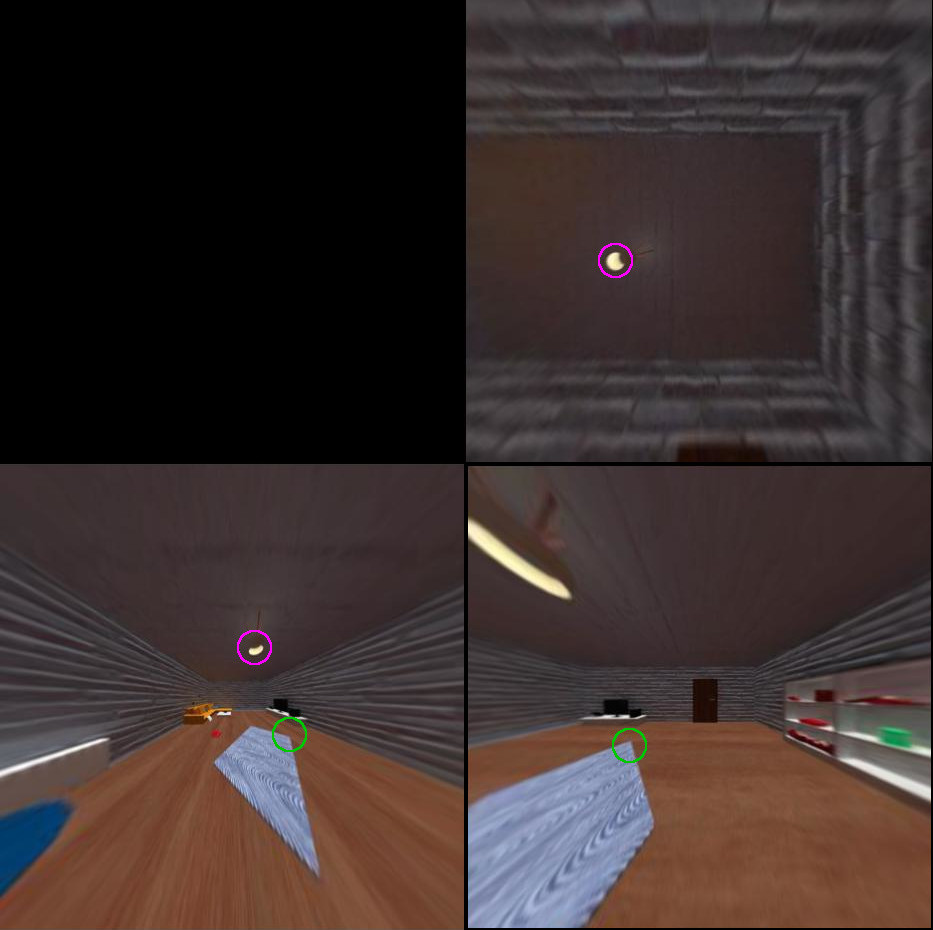
\includegraphics[width=0.9\textwidth]{03/flow_seams_ext16.jpg}
            \caption{Viewpoint A in extended cube map representation (150\degree FoV per face)}
    \end{subfigure}%
    \hfill
     %add desired spacing between images, e. g. ~, \quad, \qquad etc.
      %(or a blank line to force the subfigure onto a new line)
    \begin{subfigure}[t]{0.5\textwidth}
            \centering
            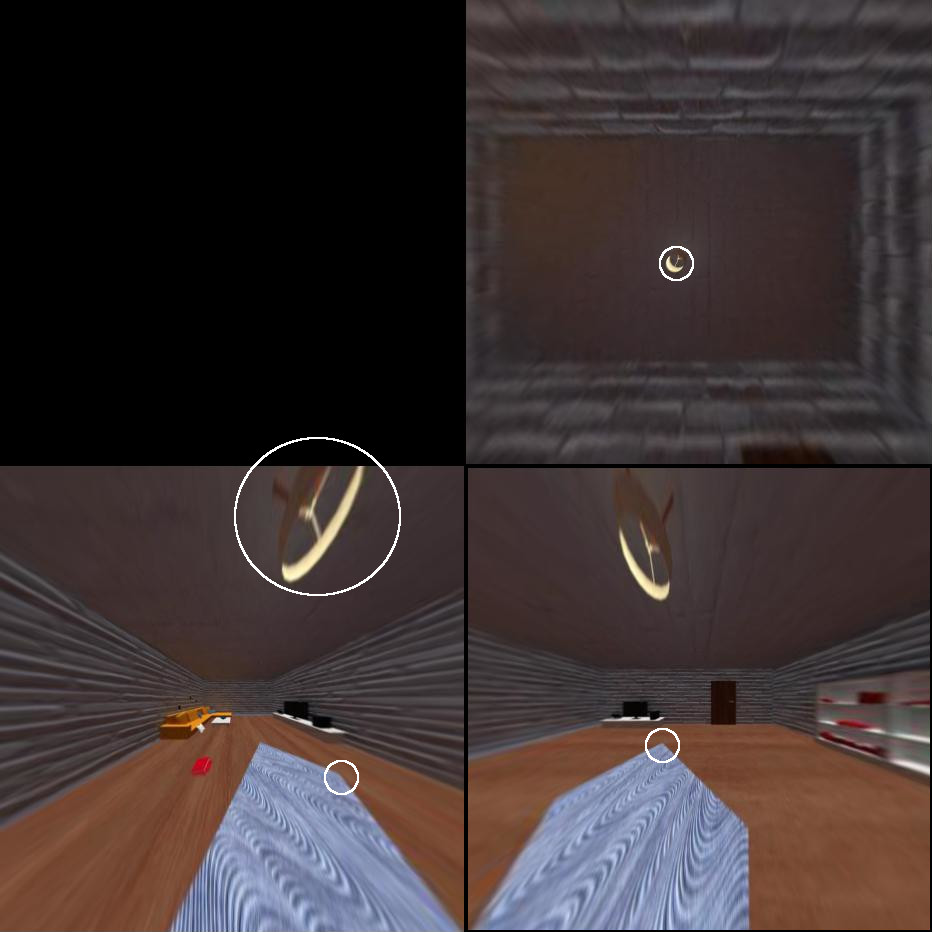
\includegraphics[width=0.9\textwidth]{03/flow_seams_ext15.jpg}
            \caption{Viewpoint B in extended cube map representation (150\degree FoV per face)}
    \end{subfigure}
    \hfill
    \hfill
  \caption[Tracking points across seams in the extended cube map]{Points that traversed a seam in the regular cube map can be tracked across the original seams in the extended cube map} \label{fig:flow_seams_ext}
\end{figure}

Nonetheless, this method is still limited by the field of view used by the virtual cameras. If the maximum displacement is larger than the face extension, the extended cube map will not be sufficient, as the points can also traverse the extended seams. Also, the larger the field of view, the more the image will be distorted towards the edges of a face, which may lead to distorted optical flow results. Both problems are visible in Figure~\ref{fig:flow_seams_ext}: The lamp in the left face has such a large displacement between a and b that it is partly cut off in b. On top of being cut off, it is also greatly distorted, which will result in distorted optical flow values for that area.

In general, this means that displacement between two images is limited. However, the displacement that is trackable by optical flow algorithms is also limited. The effect of these limitations will be explored in Chapter~\ref{chap:evaluation}.

Despite these limitations, using the extended cube map makes it possible to calculate optical flow on each face separately, meaning that Megastereo's flow-based blending method can be applied to two 360\degree viewpoints A and B: First, the extended cube map projections $A_{ext}$ and $B_{ext}$ are created from the image data. From this point, each set of faces $A_{ext}^{i}$ and $B_{ext}^{i}, i \in [top, left, front, right, bottom, back]$ is handled separately. Optical flow $F_{A\to B}^i$ and inverse optical flow $F_{B\to A}^i$ are calculated for $A_{ext}^{i}$ and $B_{ext}^{i}$. Then, the shifted image is calculated using Equation~\ref{eq:flow_blending}. Finally, for each face, the extended parts of the extended cube map are clipped so that each face once again has a field of view of 90$^{\circ}$, resulting in the blended 360\degree image at position $\delta$ between viewpoints A and B. Since the flow-based blending method is applied to two complete images instead of image strips like in Megastereo, it is equivalent to interpolation with one degree of freedom (i.e. on a line) between viewpoints A and B. This interpolated viewpoint can then be used for texture lookup just like a captured viewpoint.

\subsubsection{2DoF Synthesis with Flow-based Blending} \label{subsec:2dof_flow-based}
Adapting Megastereo's flow-based blending for 1DoF interpolation of 360\degree images allows the creation of a new viewpoint between A and B that is closer to the actual ray (Figure~\ref{fig:flow-based-mot}b). In order to leverage this to improve the basic 2DoF synthesis, the 1DoF interpolation needs to be integrated in the 2DoF synthesis algorithm. For each pixel of the synthesized image, a set of input viewoints A and B needs to be chosen for use in the 1DoF interpolation. Then, based on the positions of A and B, and the ray in question, an interpolation distance $\delta$ must be calculated that defines the position of the 1DoF interpolation between A and B.

For these steps, an approximation needs to be made due to the 2DoF restriction: Figure~\ref{fig:flow_simplification-mot}a and b show the ideal case, where the target point $T$ is on the same horizontal plane as the captured points and the synthesized point (the viewpoint plane). In this case there are a number of different positions directly on the ray that are also on the plane. Depending on the input viewpoints, the most convenient can be chosen and an interpolated viewpoint calculated at that position. However, this is only the case for all target points \emph{on this plane}. All other target points in the scene lie either above or below the viewpoint plane, for example in Figure~\ref{fig:flow_simplification-mot}c, where T is above the plane. In these cases, the only intersection of the ray and the viewpoint plane is at the synthesized viewpoint. Finding the set of viewpoints A and B that allow the closest 1DoF interpolation to this point is not trivial, as it would require comparing the minimum distance of the point to all vectors between all the possible sets of viewpoints. In order to simplify this problem, all the rays that are not on the viewpoint plane are approximated.

To approximate a ray pointing at target point T at the spherical coordinates $(r, \theta, \varphi)$, the elevation $\theta$ is reduced to 0, assigning the spherical coordinates to $(r, 0, \varphi)$, which is equivalent to moving T to the viewpoint plane by the shortest path. This will yield less accurate results as the actual ray moves towards the poles, since the deviation angle between the actual ray and the approximated ray increases towards the poles. However, this approximation is computationally and mathematically much simpler and should yield acceptable results.

\begin{figure}
\centering
    \hfill
    \begin{subfigure}[t]{0.3\textwidth}
            \centering
            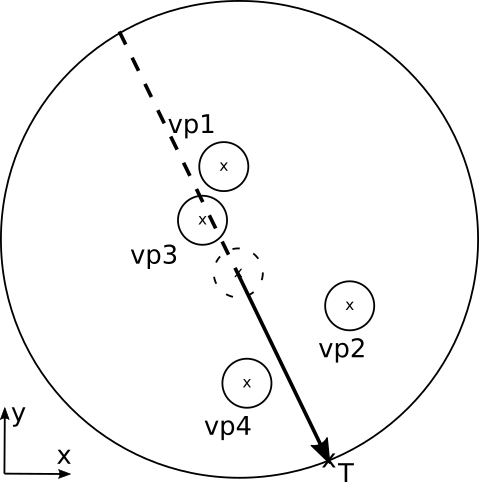
\includegraphics[width=0.9\textwidth]{03/flow_simplification01.png}
            \caption{Scene view from above: The target point T is on the viewpoint plane}
    \end{subfigure}%
    \hfill
    \begin{subfigure}[t]{0.3\textwidth}
            \centering
            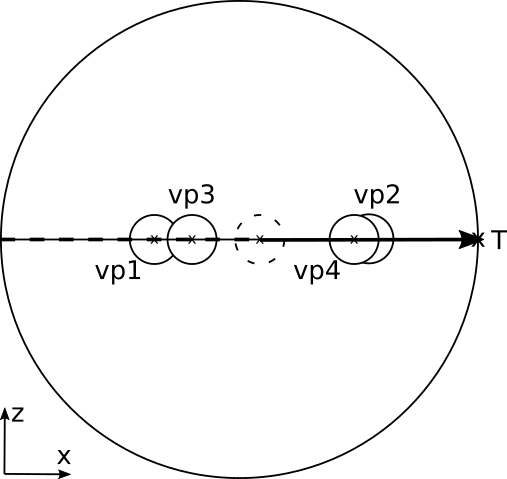
\includegraphics[width=0.95\textwidth]{03/flow_simplification02.png}
            \caption{Scene view from the side: The target point T is on the viewpoint plane}
    \end{subfigure}
    \hfill
    \begin{subfigure}[t]{0.3\textwidth}
            \centering
            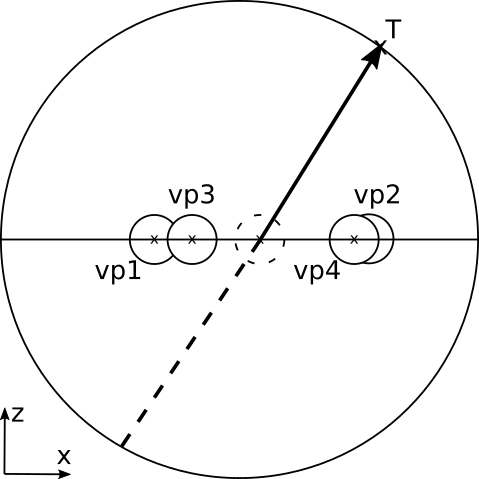
\includegraphics[width=0.9\textwidth]{03/flow_simplification03.png}
            \caption{Scene view from the side: The target point T can also be above (or below) the viewpoint plane}
    \end{subfigure}%
    \hfill
    \hfill
  \caption{Example of different target points in the scene} \label{fig:flow_simplification-mot}
\end{figure}

With this approximation, the viewpoints A and B used for 1DoF interpolation can be chosen. As in basic 2DoF synthesis, the metric for choosing A and B is the deviation angle. The actual rays, not the approximated rays, are used for the calculation and comparison of the deviation angles, since there is no need to use the approximated rays at this point. However, for the choice of A and B, an additional constraint is included: The two viewpoints chosen must be on either side of the approximated ray, so that there is an intersection between the vector connecting the viewpoints A and B and the approximated ray (see Figure~\ref{fig:flow_vpchoice}).

\begin{figure}
\centering
    \hfill
    \begin{subfigure}[t]{0.3\textwidth}
            \centering
            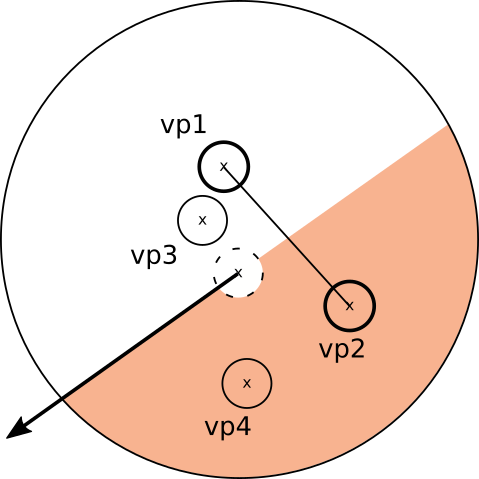
\includegraphics[width=0.9\textwidth]{03/flow-vpchoice01.png}
            \caption{A: vp1, B: vp2}
    \end{subfigure}%
    \hfill
    \begin{subfigure}[t]{0.3\textwidth}
            \centering
            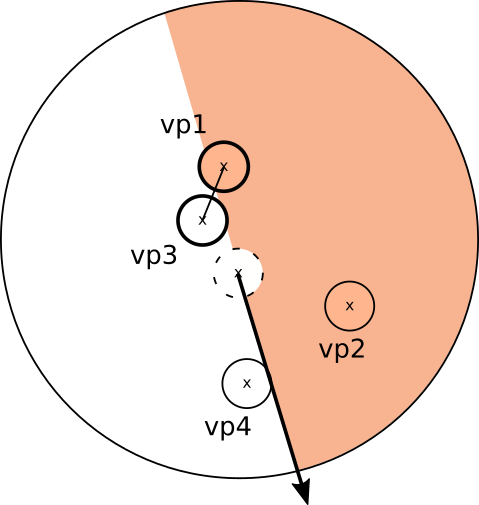
\includegraphics[width=0.9\textwidth]{03/flow-vpchoice02.png}
            \caption{A: vp1, B: vp3}
    \end{subfigure}
    \hfill
    \begin{subfigure}[t]{0.3\textwidth}
            \centering
            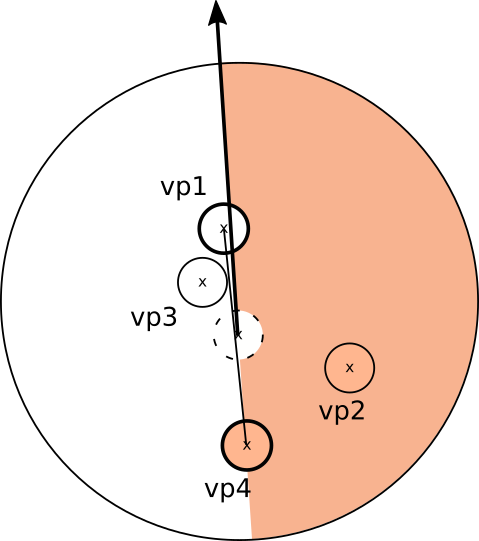
\includegraphics[width=0.9\textwidth]{03/flow-vpchoice03.png}
            \caption{A: vp1, B: vp4}
    \end{subfigure}%
    \hfill
    \hfill
  \caption[Examples of the choice of viewpoints A and B for 1DoF interpolation]{Examples of the choice of viewpoints A and B for 1DoF interpolation based on deviation angle and position on either side of the ray. The two sides of the ray are color coded in white and orange.} \label{fig:flow_vpchoice}
\end{figure}

Once the viewpoints A and B are chosen for each target point T, the interpolation distance $\delta \in [0,1]$ is calculated, which is the the point on the vector $\overrightarrow{AB}$ that intersects the approximated ray. The calculation of $\delta$ is a simple line intersection calculation, explained in Section \ref{sec:impl_details}.

Using the chosen viewpoints A and B, and the calculated interpolation distance $\delta$, a 1DoF interpolation is calculated for each approximated ray. Using this interpolated viewpoint, a texture lookup is then performed for each pixel associated with that ray. This results in a mosaicked image where each image area (vertical strip in equirectangular representation) is an interpolated, reprojected viewpoint. The 1DoF interpolation step should improve some of the artefacts caused by the use of the model sphere instead of the actual scene geometry. Its effectiveness and limitations are explored in Chapter~\ref{chap:evaluation}.

\section{Implementation Details} \label{sec:impl_details}
This section presents the technical and mathematical details on which the basic 2DoF synthesis and the 2DoF synthesis with flow-based blending are based. 
The basic 2DoF synthesis and the 2DoF synthesis with flow-based blending are implemented in Python3 \cite{python}, using the libraries NumPy \cite{numpy}, OpenCV \cite{opencv}, SciPy \cite{scipy}, and scikit-image \cite{skimage}. For the conversion between different 360\degree projections, as well as the calculation of the extended cube map, the library ``skylibs'' \cite{skylibs} is used.

\missingfigure{2DoF process diagram}

\subsection{Preprocessing}
The input data consists of a set of captured viewpoint images in equirectangular representation, a text file containing the metadata (positions and orientations) of these viewpoints, and the approximate scene radius. In order to easily and intuitively access the locations and image data of the captured viewpoints, the data is encapsulated in the CaptureSet class. The CaptureSet class first parses the metadata, then, with this information, rotates all the images so that they have the same orientation, and shifts the viewpoint cloud so that it is centered around the origin (0,0,0). This is done under the assumption that images were captured in a regular distribution throughout the room. The model sphere representing the scene is also centered at the origin. Instead of storing the image data directly in the CaptureSet, the file paths are stored so that the images can be dynamically loaded when needed. The CaptureSet can then be used by the ImgSynthesizer to synthesize a new image either using regular blending or flow-based blending at any given location within the scene\footnote{Given that it is within the convex hull of the captured viewpoints}.

\subsection{Basic 2DoF Synthesis}
For the basic 2DoF Synthesis, the steps described in detail in this section are the calculation of the ray-scene intersection and the texture lookup, as well as the deviation angle calculation and blending function introduced in Section~\ref{subsec:basic-synthesis}.

%\subsubsection{Selecting Appropriate Input Viewpoints}
%Before calculating ray-scene intersections and performing texture lookup, the most appropriate input viewpoints are selected from the complete set of input viewpoints. Since resolution does play a role in the resampling, 

\subsubsection{Calculating Ray-sphere Intersection}
The ray-sphere intersection is used in the raytracing-based texture lookup to find the scene points captured by the synthesized viewpoint (see \ref{fig:raytracing}c). This raytracing process is a basic raytracing technique used in computer graphics. The vectors representing the rays of a viewpoint can be easily derived from the world coordinates of the 360\degree image (see~Section~\ref{subsec:fundamentals_360}): Each point of the world coordinates is a vector on the unit sphere, representing the location of an image value (pixel). These coordinates are in \emph{model space}, meaning that they are centered around zero. Translating them into \emph{world space} moves the rays to their respective location in the scene, where the vectors represent the rays cast into the scene, where they will intersect with the model geometry.

The intersections of these rays with the model sphere can be calculated analytically: The model sphere, which is centered at the origin, can be represented implicitly by Equation~\ref{eq:rsi_spherefull}. The set of points P defined by this equation make up the surface of the sphere (Equation~\ref{eq:rsi_sphereP}). 
The equation describing any point on the ray can be expressed by Equation~\ref{eq:rsi_point}, where $O$ is the origin of the ray, which is the center of projection of the new viewpoint, $t$ is the length of the ray and $D$ is a unit vector describing the direction. 

\begin{align}
  x^2 + y^2 + z^2 - R^2 = 0&\label{eq:rsi_spherefull}\\ 
  P^2 - R^2 = 0&\label{eq:rsi_sphereP}
\end{align} 
\begin{align}
  P = O + tD& \label{eq:rsi_point}
\end{align} 

The point $P$ in Equation~\ref{eq:rsi_sphereP} can be substituted with the equation of the any point on the ray which yields Equation~\ref{eq:rsi_sub}. This equation can be developed into Equation~\ref{eq:rsi_quad}, which is a quadratic function with $a = D^2$, $b = 2OD$, $c = O^2-R^2$ (Equation~\ref{eq:quadf}).

\begin{align}
  |O + tD|^2 - R^2 &= 0  \label{eq:rsi_sub}\\
  D^2 t^2 + 2ODt + O^2 - R^2 &= 0 \label{eq:rsi_quad}
\end{align}

\begin{align}
  a = D^2, b = 2OD, c = O^2-R^2 \nonumber \\
  f(t) = at^2 + bt + c \label{eq:quadf}\\
  t = \frac{-b \pm \sqrt{b^2 - 4ac}}{2a} \label{eq:solvequadf}
\end{align}

This equation can then be solved for t. Since the radius of the sphere is chosen so that it contains the complete scene and no viewpoints are synthesized outside of the scene, the quadratic function will always have two solutions (i.e. two intersections): one for which the vector length $t$ is negative, and one for which the vector length is positive. Since the original ray used for the calculation is unidirectional (i.e. it cannot invert its direction), it needs to be extended by a positive value. The original ray, being a unit ray of length 1, can then be multiplied by the positive $t$, which yields the intersection point. 

The vectors and intersection points are each calculated and stored in latlong representation (i.e. matrix of vectors of the same shape as the latlong image), which means that they can handily be associated with the world coordinates, as well as the uv coordinates (and thus, pixel values) using the latlong mapping function. By storing the values in this representation (i.e. 3D matrix), Numpy's vectorization can be used, which greatly facilitates implementation.

\subsubsection{Texture Lookup}
The texture lookup shown in Figure~\ref{fig:raytracing}d-f is performed by resampling using uv coordinates. Given a captured viewpoint at the location V and the ray-scene intersections from the synthesized viewpoint $T_i$, where $i$ denotes which ray is being examined, the rays from the V to the intersections can easily be calculated by $T_i-V$ (see Figure~\ref{fig:impl_texture_lookup}a). These rays are then normalized to have length 1 and returned to model space (see Figure~\ref{fig:impl_texture_lookup}b). The normalized rays in model space are then transformed from world coordinates to image coordinates. These image coordinates (i.e. uv coordinates) can be used to resample the data, which is equivalent to actually performing a ray-by-ray texture lookup, but much faster. The result of the resampling along with the ``new'' rays is shown in Figure~\ref{fig:impl_texture_lookup}c. This resampling based on uv coordinates is implemented in the library Skylibs \cite{skylibs} and utilizes Scipy's function \emph{scipy.ndimage.map\_coordinates}.

\begin{figure}
\centering
    \hfill
    \begin{subfigure}[t]{0.3\textwidth}
            \centering
            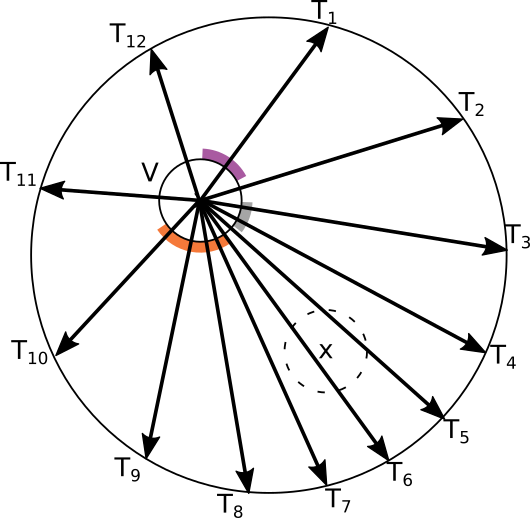
\includegraphics[width=0.9\textwidth]{03/impl_texture_lookup01.png}
            \caption{The rays $T_i-V$ in world space}
    \end{subfigure}%
    \hfill
    \begin{subfigure}[t]{0.3\textwidth}
            \centering
            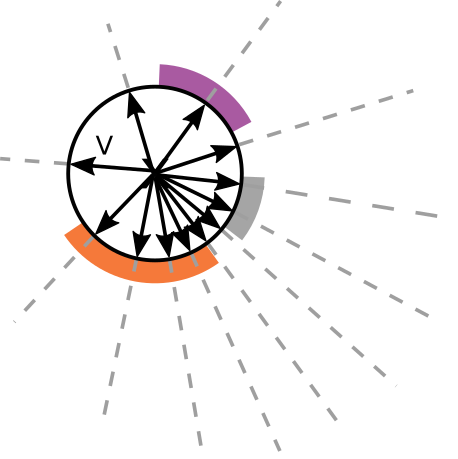
\includegraphics[width=0.9\textwidth]{03/impl_texture_lookup02.png}
            \caption{The normalized rays $T_i-V$ in model space}
    \end{subfigure}
%    \hfill
%    \begin{subfigure}[t]{0.19\textwidth}
%            \centering
%            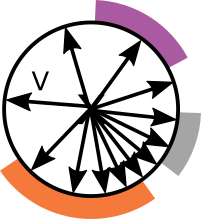
\includegraphics[width=0.9\textwidth]{03/impl_texture_lookup03.png}
%            \caption{}
%    \end{subfigure}%
    \hfill
    \begin{subfigure}[t]{0.3\textwidth}
            \centering
            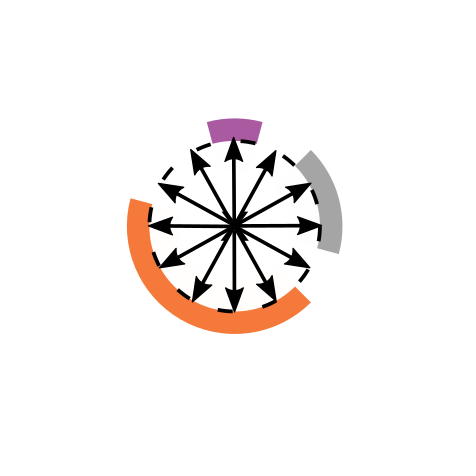
\includegraphics[width=0.9\textwidth]{03/impl_texture_lookup04.png}
            \caption{The result of resampling based on uv coordinates}
    \end{subfigure}%
    \hfill
  \caption{Texture lookup by uv remapping} \label{fig:impl_texture_lookup}
\end{figure}

\subsubsection{Deviation Angle Calculation and Knn Blending}
The deviation angle calculation is a simple angle calculation between vectors. This calculation is performed for each ray of the synthesized point and the corresponding rays of all of the input viewpoints.
Again, the deviation angles per viewpoint are stored in latlong representation (Figure~\ref{fig:dev_angle_storage}a). The deviation angles for all viewpoints are stacked in a three-dimensional matrix, which allows comparison of the deviation angles per pixel/ray of all the viewpoints (Figure~\ref{fig:dev_angle_storage}b). This makes the  of the viewpoint per pixel very straightforward, since the id of the k best input viewpoints can easily be extracted and the corresponding pixel value retrieved. With this information, the ``regular'', k-nearest-neighbor (knn) blending is performed.
\todo{whyyy arent the two dev angle images not the same size??}

\begin{figure}
\centering
    \hfill
    \begin{subfigure}[t]{0.4\textwidth}
            \centering
            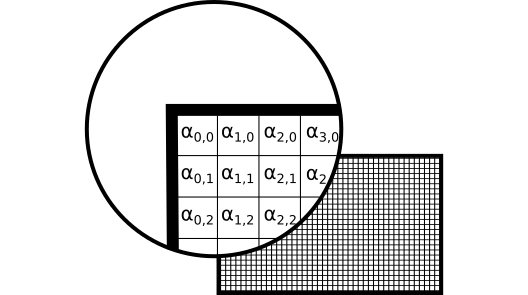
\includegraphics[width=\textwidth]{03/impl_dev_storage01.png}
            \caption{The deviation angles of one input viewpoint in latlong format}
    \end{subfigure}%
    \hfill
    \begin{subfigure}[t]{0.4\textwidth}
            \centering
            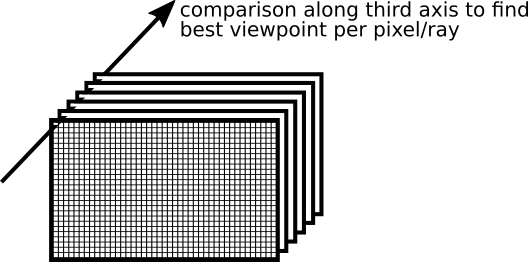
\includegraphics[width=\textwidth]{03/impl_dev_storage02.png}
            \caption{The stacked deviation angles of all input viewpoints}
    \end{subfigure}
    \hfill
  \caption{Visualization of deviation angle storage} \label{fig:dev_angle_storage}
\end{figure}

The regular blending function combines the values of the rays of the k closest deviation angles $\alpha$. The idea behind it is to weight deviation angles of 0 very highly and all larger deviation angles with exponentially low values. This is done with an inverse sigmoid function (Function~\ref{eq:sigmoid}, visualized in Figure~\ref{fig:sigmoid}). The parameters of the function were found by trial and error.

\begin{align}
  w(\alpha) = \frac{1}{(1 + e^{500\cdot(\alpha - 0.017)})} \label{eq:sigmoid}
\end{align}

\begin{figure}
		\centering
		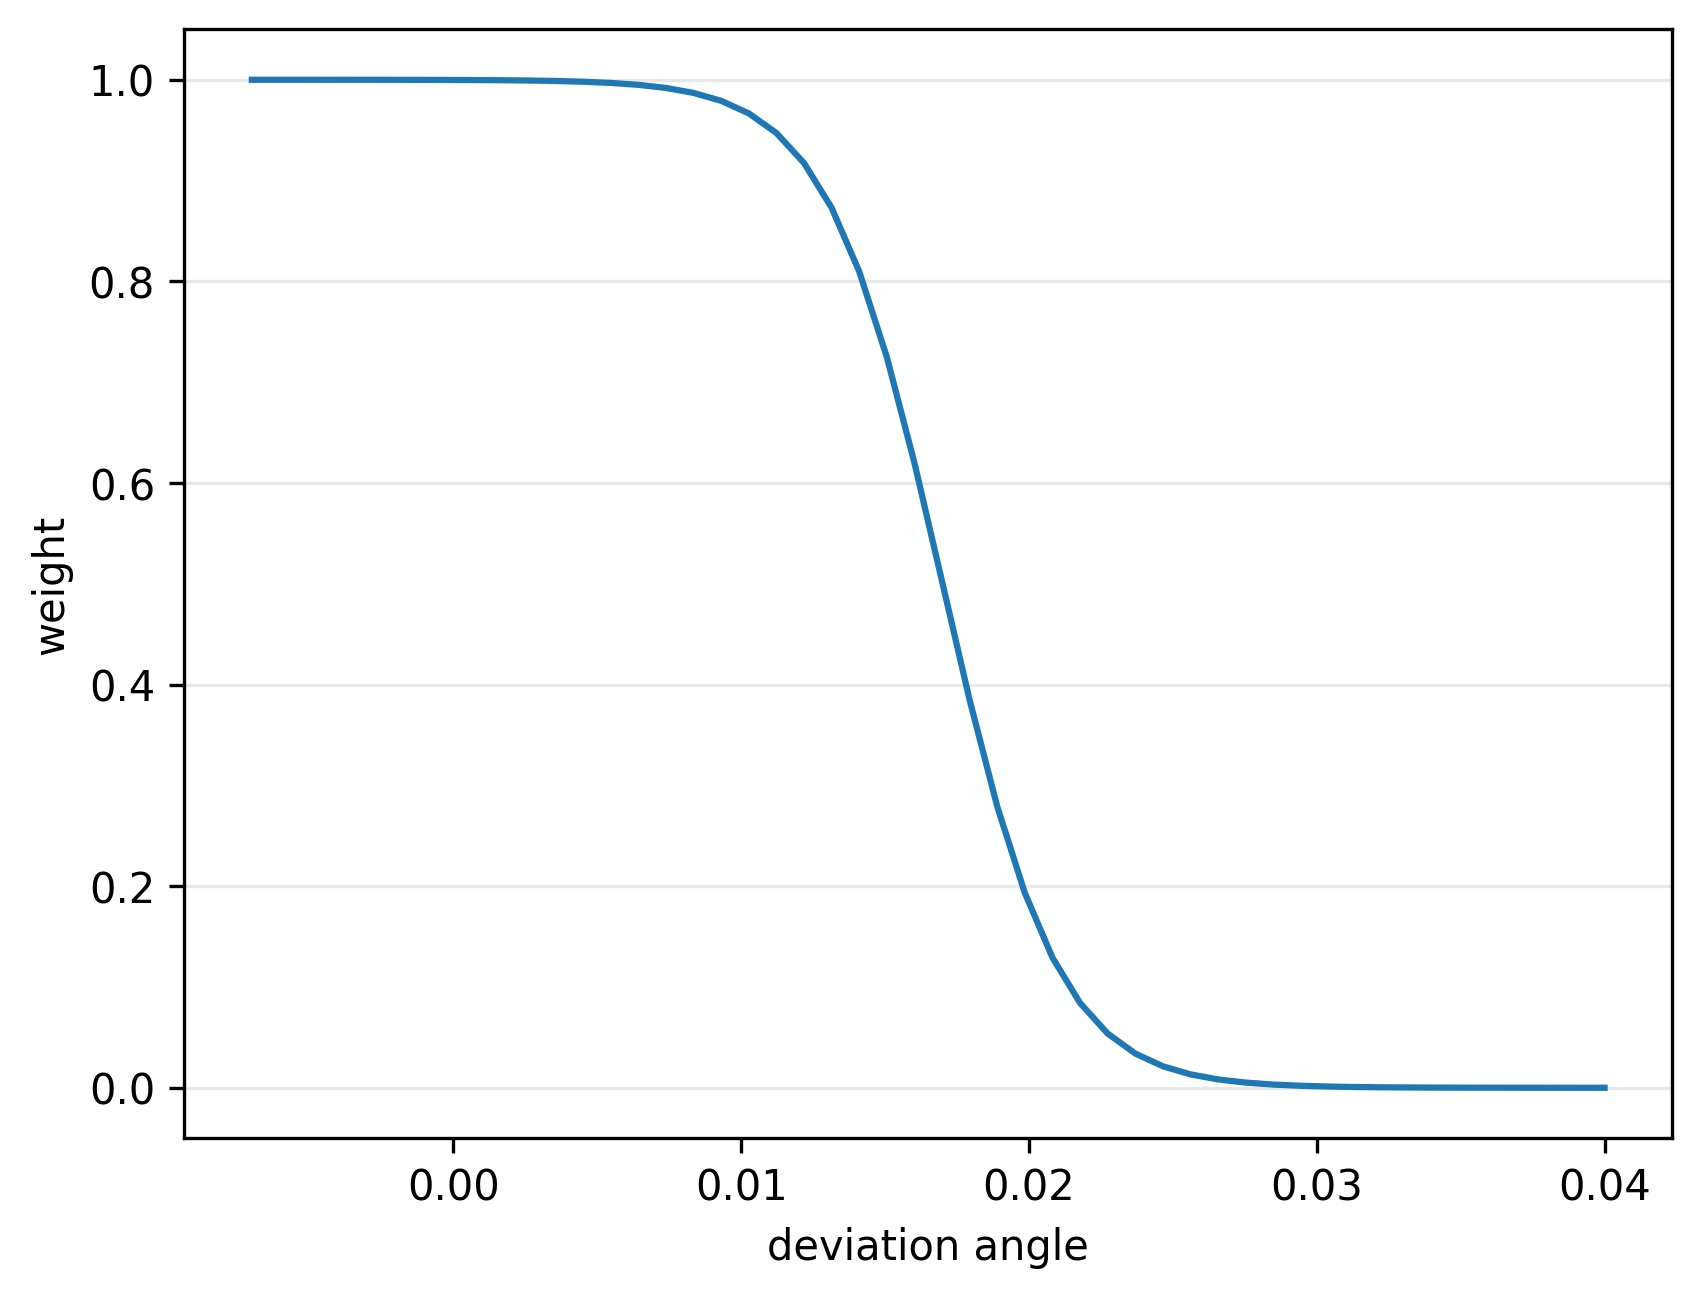
\includegraphics[width=0.5\textwidth]{03/inverse_sigmoid.jpg}
		\caption{The inverse sigmoid function used for weighting}
		\label{fig:sigmoid}
\end{figure}

Then, the per-pixel weights $w$ are normalized so that their sum for each pixel is one, so that the final image is not oversaturated. Finally, the pixel values of the different remapped viewpoints are multiplied by the normalized weights associated with that viewpoint and the weighted images \todo{latlong representation} are added up to give the final synthesized image. Figure~\ref{fig:knn} shows the difference between $k=1$ and $k=2$. Blending the two best viewpoints per pixel results in smoother transitions between the mosaicked areas. Using $k>2$ does not have much impact, since most deviation angles where $k>3$ are too large to have an effect.

\begin{figure}
\centering
    \hfill
    \begin{subfigure}[t]{0.5\textwidth}
            \centering
            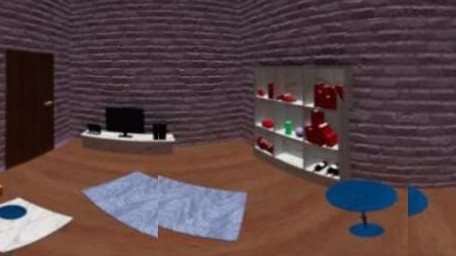
\includegraphics[width=0.9\textwidth]{03/C_max_vps_knn1.jpg}
            \caption{$k=1$}
    \end{subfigure}%
    \hfill
    \begin{subfigure}[t]{0.5\textwidth}
            \centering
            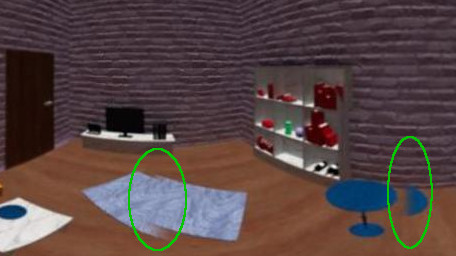
\includegraphics[width=0.9\textwidth]{03/C_max_vps_knn2.jpg}
            \caption{$k=2$}
    \end{subfigure}
    \hfill
  \caption{K-nearest-neighbor blending with different values for k} \label{fig:knn}
\end{figure}

\subsection{Flow-based Blending}
The 2DoF synthesis with flow-based blending utilizes some steps from the basic 2DoF synthesis, such as the deviation angle calculation and the texture mapping. The details of the choice of viewpoints A and B for the 1DoF interpolation, the calculation of the interpolation distance $\delta$, as well as the 1DoF intepolation are explained in this section. 

\subsubsection{Choosing the Viewpoints A and B}
The choice of the input viewpoints A and B for the 1DoF interpolation is important in that two viewpoints need to be chosen that are on either side of the ray in question (see Figure~\ref{fig:flow_vpchoice}), so that the line on which the images can be interpolated actually intersects the ray. Since all the viewpoints are on a plane, the ``side'' a viewpoint is on is defined by the sign of the deviation angle. Instead of just calculating the angle between the two rays


\subsubsection{Determining the 1DoF Interpolation distance $\delta$}
Given the two viewpoints A and B, it is now possible to calculate the intersection of $\overrightarrow{AB}$ and the approximated ray (elevation $\theta = 0$) between the synthesized point $S$ and the target point $P$ in the scene (Figure~\ref{fig:flow_pos}). The calculation of the intersection between two lines is a simple method based\ldots\todo{either cite or declare as common knowledge} Using these four points A,B,P and S, two infinite lines can be defined (Equation~\ref{eq:lines}). The intersection point at $t * \overrightarrow{AB}$ is given by Equation~\ref{eq:t}.
%Like in basic 2DoF synthesis, having only two input viewpoints A and B trivializes the choice of viewpoints for flow-based blending. For any point in the scene, the ray from the synthesized point is retrieved (same as in basic 2DoF synthesis). However, instead of a texture lookup, the distance factor $\delta \in [0,1]$ of the interpolated viewpoint $vp_{AB}$ is calculated.

\begin{align}
  \overrightarrow{AB} = A + t * (B-A) \quad \overrightarrow{SP} = S + u * (P-S) \label{eq:lines} \\
  t = \frac{(x_A - x_S)(y_S - y_P) - (y_A - y_S)(x_S - x_P)}{(x_A - x_B)(y_S - y_P) - (y_A - y_B)(x_S - x_P)} \label{eq:t}
\end{align}

When t is $\in [0,1]$ (meaning there is an intersection between between A and B), it can be used directly as the interpolation distance $\delta$. However, it is possible that no viewpoints A and B exist, where \ldots is this really possible? what to do with min vps calculation?

- we are in the convex hull, so min vps is ok

%- selection of a viewpoint ``on either side'' \ar what if the viewpoint on one side has a very large deviation angle or does not exist?
%- can it not exist if we are looking at the convex hull? Yes, if the point is exctly on the border
%- possible solution: if none is found, use only one side

\begin{figure}
\centering
    \hfill
    \begin{subfigure}[t]{0.33\textwidth}            
            \centering
            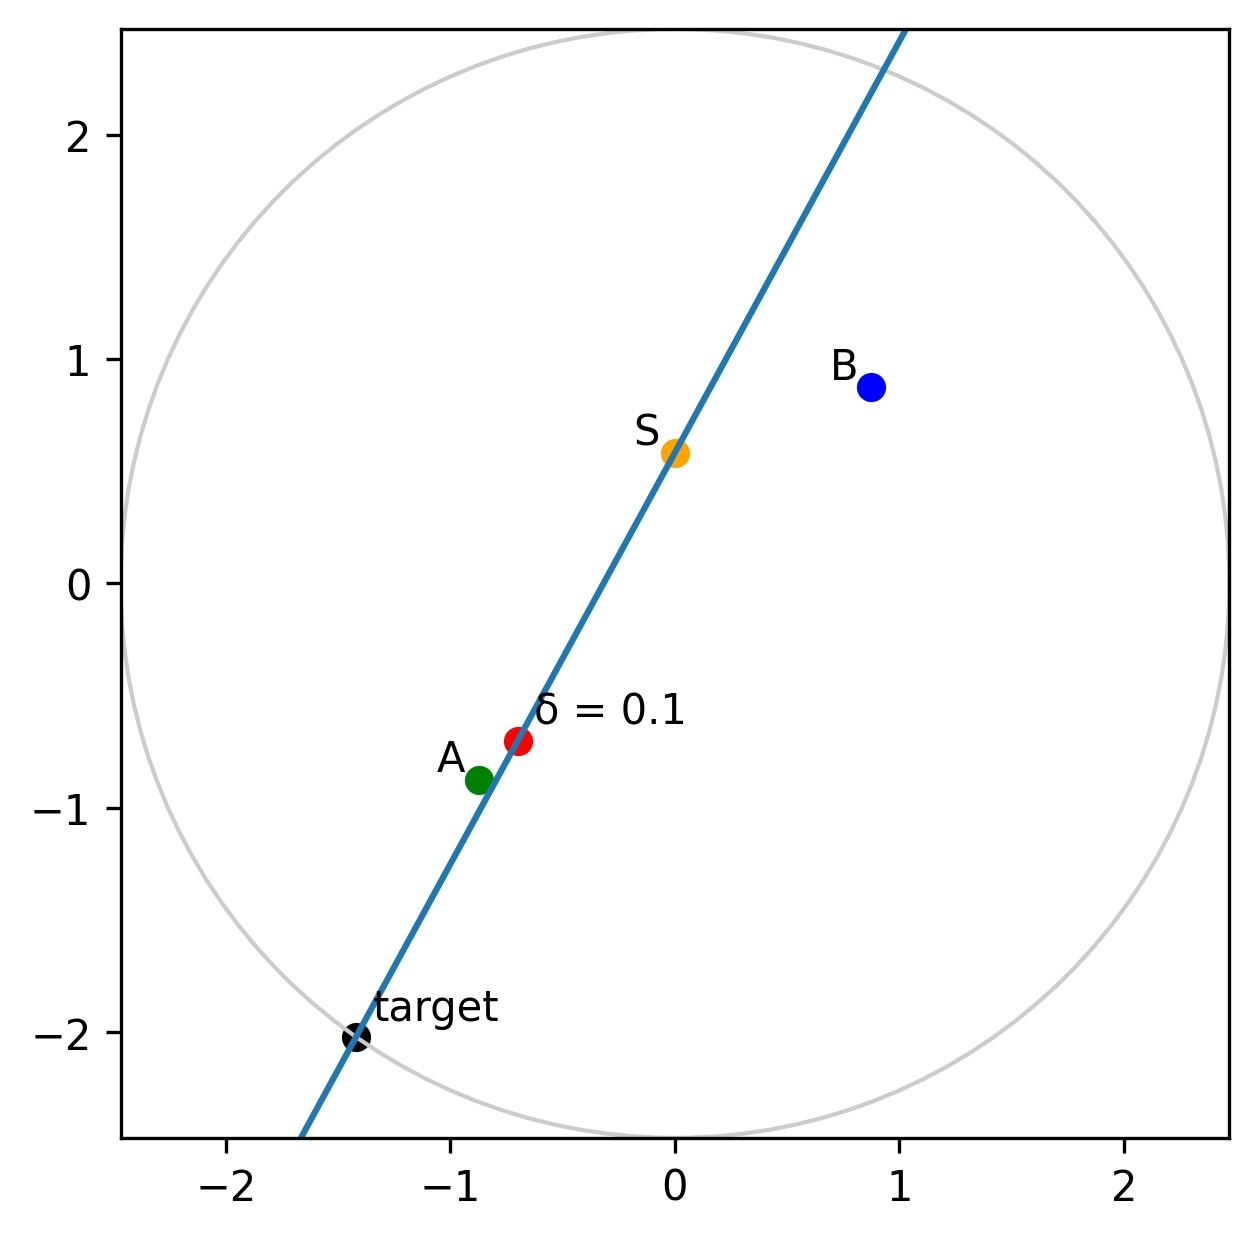
\includegraphics[width=\textwidth]{03/flow_pos420.jpg}
            \caption{}
    \end{subfigure}%
    \hfill
     %add desired spacing between images, e. g. ~, \quad, \qquad etc.
      %(or a blank line to force the subfigure onto a new line)
    \begin{subfigure}[t]{0.33\textwidth}
            \centering
            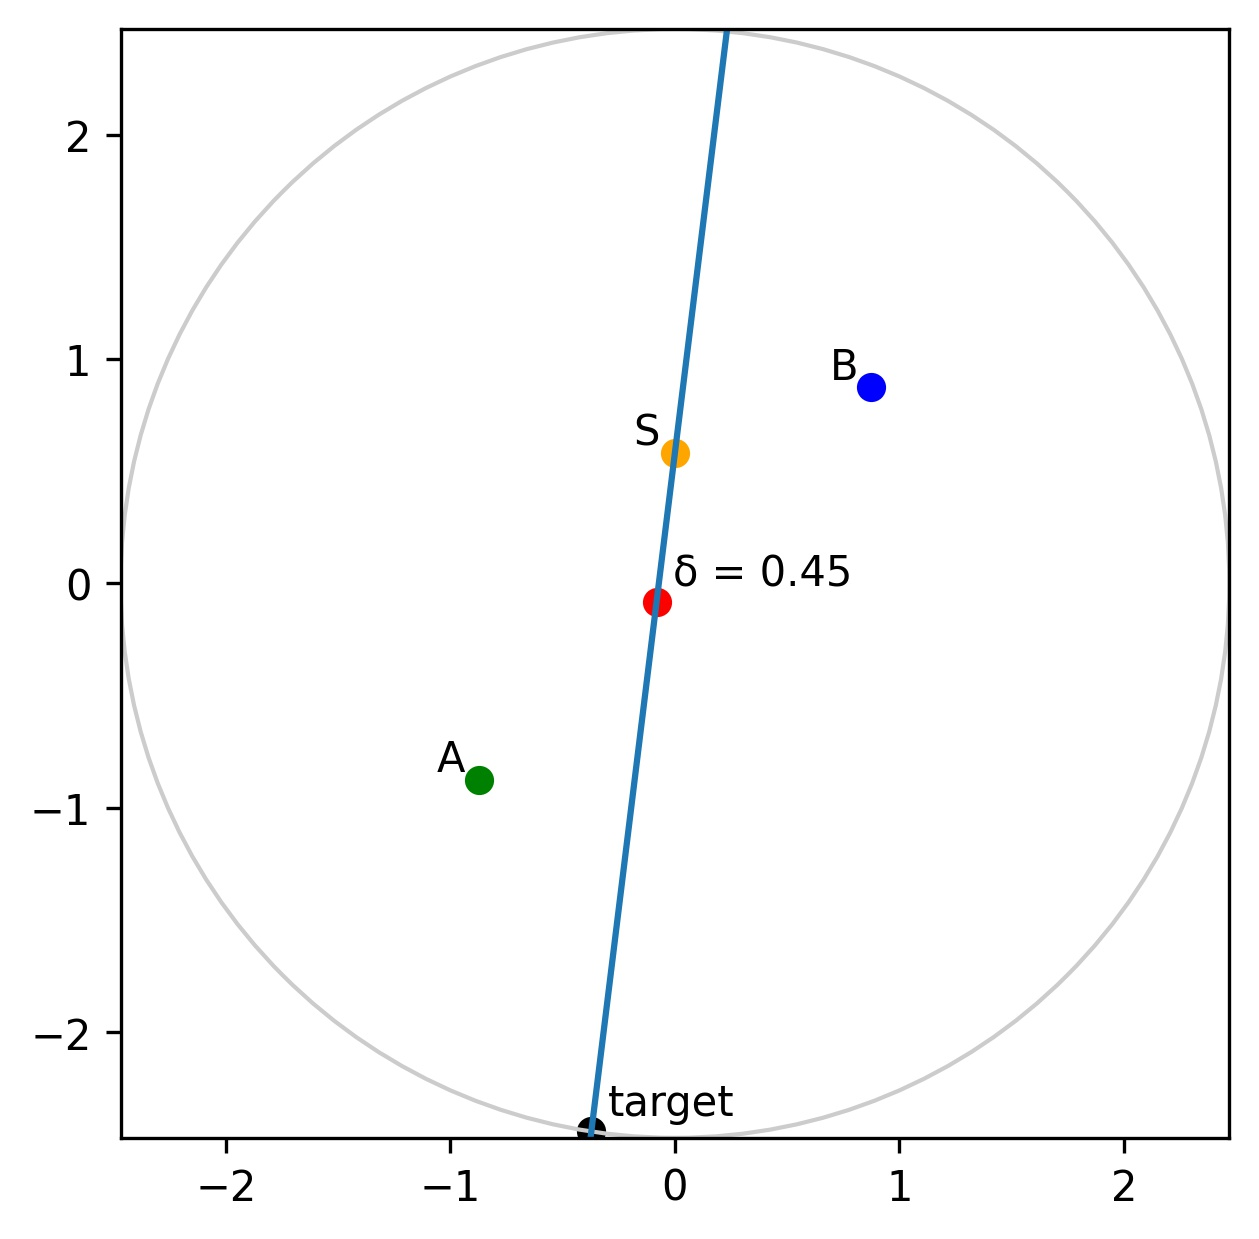
\includegraphics[width=\textwidth]{03/flow_pos480.jpg}
            \caption{}
    \end{subfigure}
    \hfill
    \begin{subfigure}[t]{0.33\textwidth}
            \centering
            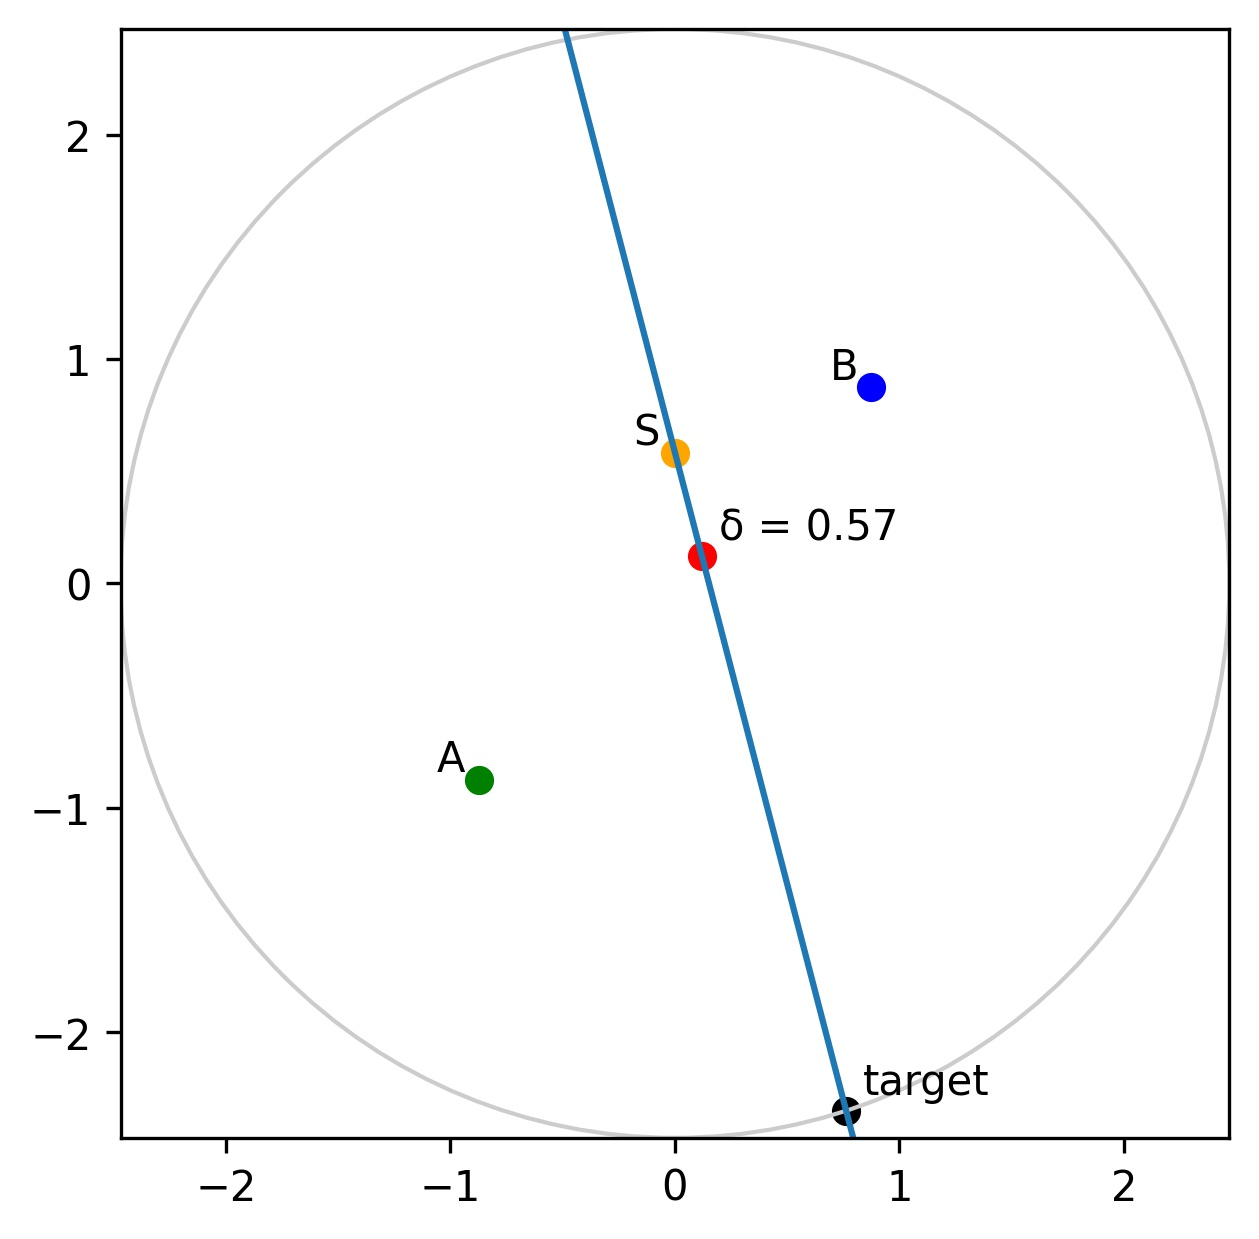
\includegraphics[width=\textwidth]{03/flow_pos540.jpg}
            \caption{}
    \end{subfigure}
    \hfill
    \caption[Different examples of $\delta$]{Depending on the scene point, a different $\delta$ is calculated based on the intersection of $\overrightarrow{AB}$ and $\overrightarrow{S,target}$} \label{fig:flow_pos}
\end{figure}

\subsubsection{1DoF Interpolation}
Given the two viewpoints A and B and the interpolation distance $\delta$, the interpolated image at $\delta$ between A and B can be calculated. The different steps of the process are extending the cube map, calculating optical flow on the extended cube map, shifting the images by the optical flow, and transforming the shifted, extended cube map back into latlong representation so that it can be remapped used for blending.
\missingfigure{1DoF process diagram}

\paragraph{Extended Cube Map}
The class \emph{ExtendedCubeMap} uses the 360\degree image data and the virtual camera provided by skylibs \cite{skylibs} to ``extend'' the cube map by capturing a virtual image for each face of the cube with a 150\degree field of view. This is done for both viewpoints A and B. The \emph{ExtendedCubeMap} class handles the extended faces and can perform different functions on them, for example the optical flow calculation, which is required for the next step.

\paragraph{Optical Flow Calculation and Image Shifting}
The optical flow algorithm used in the implementation is Farneb\"ack's algorithm implemented by OpenCV (\emph{cv2.calcOpticalFlowFarneback}) \cite{opencv}. For calculating optical flow between two \emph{ExtendedCubeMaps} A and B, the \emph{ExtendedCubeMap} class provides a function \emph{optical\_flow}, which takes as arguments the optical flow algorithm\todo{put in replaceability, possibly in future work}, and a second \emph{ExtendedCubeMap} to use for optical flow calculation. The \emph{ExtendedCubeMap} then calculates the optical flow \emph{separately} between each corresponding pair of extended faces. On top of the optical flow from \emph{ExtendedCubeMaps} A to B, the inverse optical flow from \emph{ExtendedCubeMaps} B to A is required as well. The inversion of optical flow is nontrivial\todo{maybe illustrate}, since inverting the optical flow vectors is not enough: The vectors must be shifted by their identity and then reversed. Alternatively, the optical flow can just be calculated on the \emph{ExtendedCubeMaps} in reverse, i.e.\ from B to A. This option is used in the proof-of-concept implementation in order to avoid bugs, and since the impact on performance is not very high for images with small resolution, which are used in Chapter~\ref{chap:evaluation}.

Using the optical flow, the inverted optical flow, and the interpolation distance $\delta$, the shifted images $I_A$ and $I_B$ are calculated seperately for each face by again using Scipy's \emph{scipy.ndimage.map\_coordinates}, with image coordinates shifted by the optical flow vectors and $\delta$, and the inverse optical flow vectors and $(1-\delta)$, respectively. The shifted \emph{ExtendedCubeMap} images are then combined by multiplying them by $(1-\delta)$ and $\delta$, respectively, and adding the pixel values. The result is an interpolated \emph{ExtendedCubeMap} at interpolation distance $\delta$.

Before passing this on to the blending step of the 2DoF synthesis, the \emph{ExtendedCubeMap} is transformed back into a regular cube map by clipping each face back to its original size and mapping the cube map back to a latlong map, since all other processing steps use the latlong format.

\subsubsection{Flow-based Blending}
%- combining slices of interpolations

\subsection{Performance}
%- no parallelization at the moment
%- O(n^2) because of per-pixel calculations
%- latlong storage maybe not best option, since there is lots of redundancy

\subsection{Limitations}
errors that are unrelated to the algorithm:
\begin{itemize}
  \item slight displacement due to ExtendedCubeMap
  \item black edges due to latlong-cube conversion
  \item these need to be taken into account (normalized out)
  \item only an issue for flow-based because flow-based uses conversion, whereas regular does not
\end{itemize}

